\section{Konzept}
Ausgehend von unseren Rechercheergebnissen haben wir unseren Fuchsjagd-Sender
folgendermaßen konzipiert.
\subsection{Versorgung}
\begin{figure}[H]
    \centering
    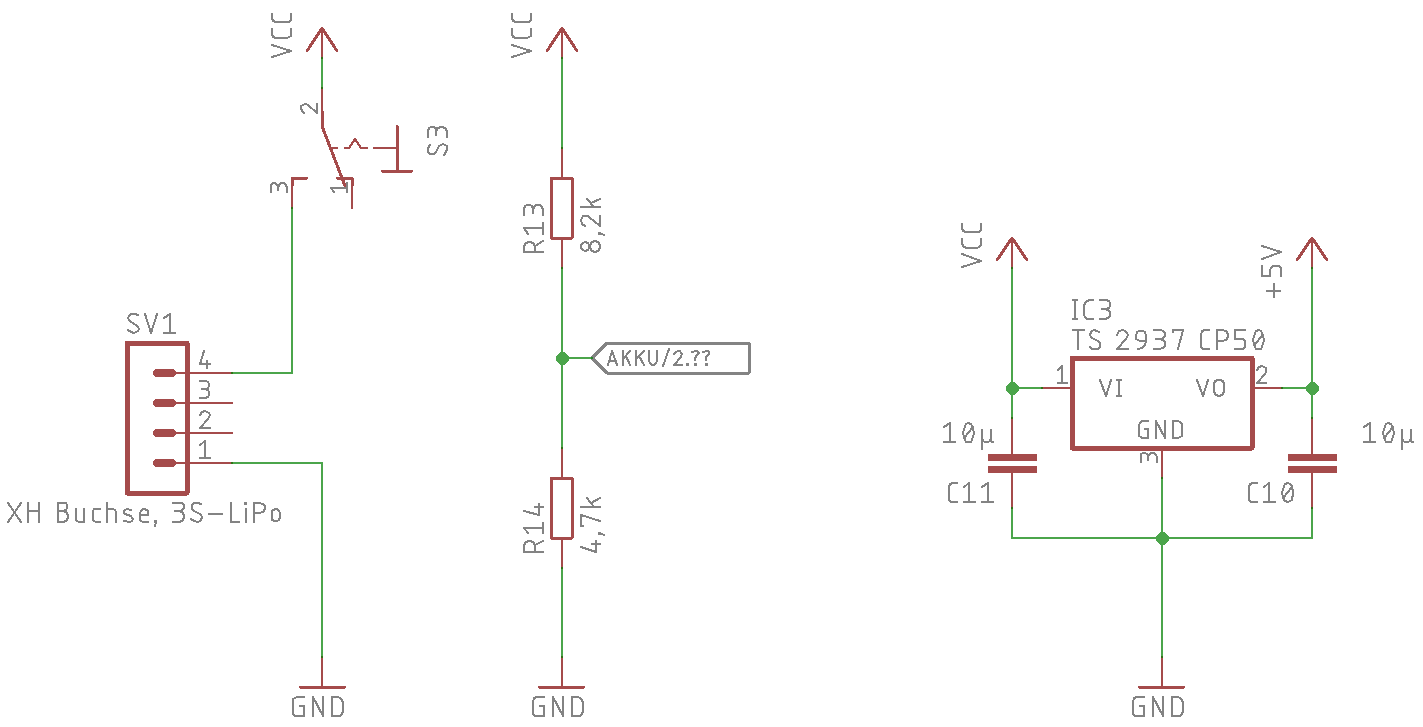
\includegraphics{res/Versorgung.png}
    \caption{Versorgung der Platine}
\end{figure}
Die Platine wird über einen dreizelligen Lithium-Ionen-Akku mit einer üblichen Nennspannung
von $11,1$V betrieben. Da unter anderem der Mikrocontroller nur mit $5$V versorgt
werden kann, nutzen wie einen Linearregler, der zusätzlich zu $12$V Schiene eine
$5$V Schiene erzeugt.

\subsection{Der Sender}
Das Sendesignal hat eine Frequenz von $3,5795$MHz und wird direkt vom auf dem Board
verbauten Quarz-Oszillator erzeugt, der zusätzlich dem Mikrocontroller als externe Clock
dient. Das erzeugte Signal lässt vom den Mikrocontroller über ein UND-Gatter steuern. Dieses
Signal wird dann letztendlich von einem FET auf $12$V verstärkt und anschließend gefiltert,
um nichtliniearitäten auszugleichen. Die Verstärkerstufe ist wie folgt aufgebaut:

\begin{figure}[H]
    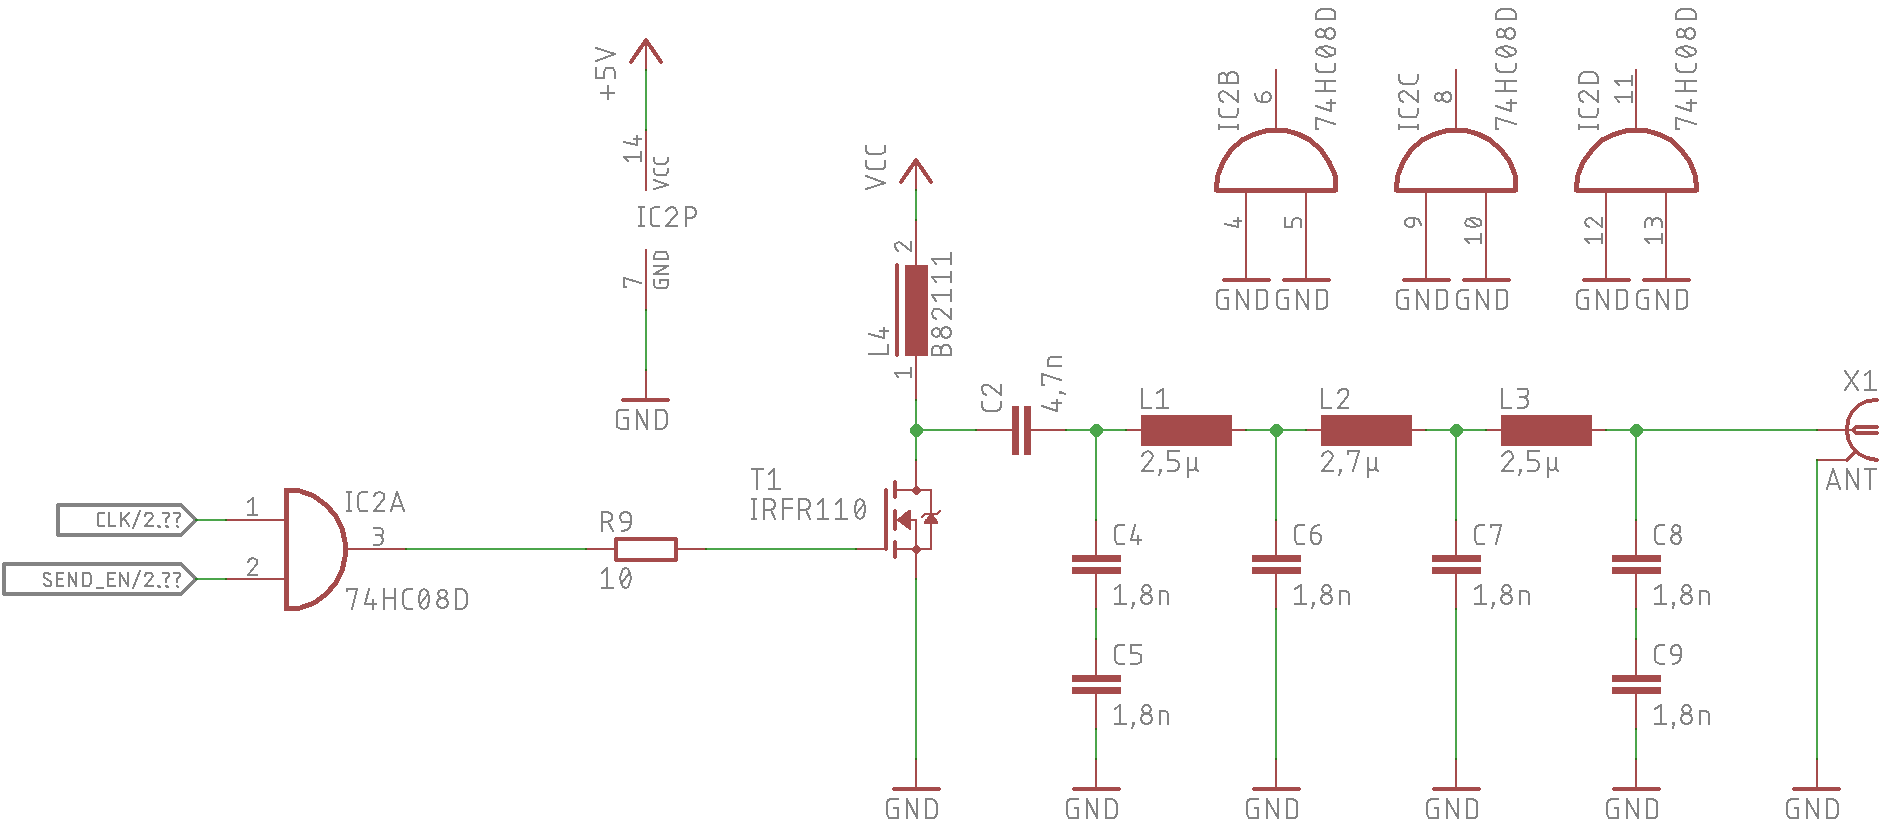
\includegraphics{res/Endstufe.png}
    \caption{Verstärkerschaltung des Senders}
\end{figure}

\subsection{Filterung des erzeugten Signals}
Damit der Sender ausschließlich im erlaubten Band sendet, wird der Verstärkerstufe
ein Tiefpassfilter nachgeschaltet. Wir haben uns für einen Tiefpassfilter siebter 
Ordnung von Typ Tschebyscheff entschieden, da er eine sehr hohe Steilheit aufweißt
und die Ripple kein Problem darstellen, da wir ohnehin ein sehr schmalbandiges
Signal senden wollen. Das Filter ist wiefolgt aufgebaut:
\begin{figure}[H]
    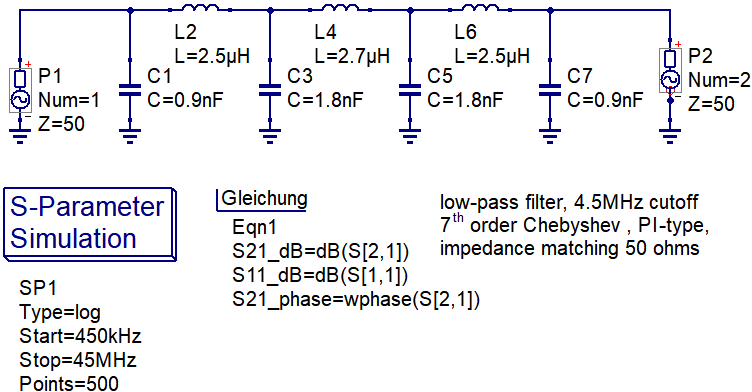
\includegraphics{res/TP_Schaltplan.png}
    \caption{Aufbau des Tschebyscheff-Filters}
\end{figure}

\begin{figure}[H]
    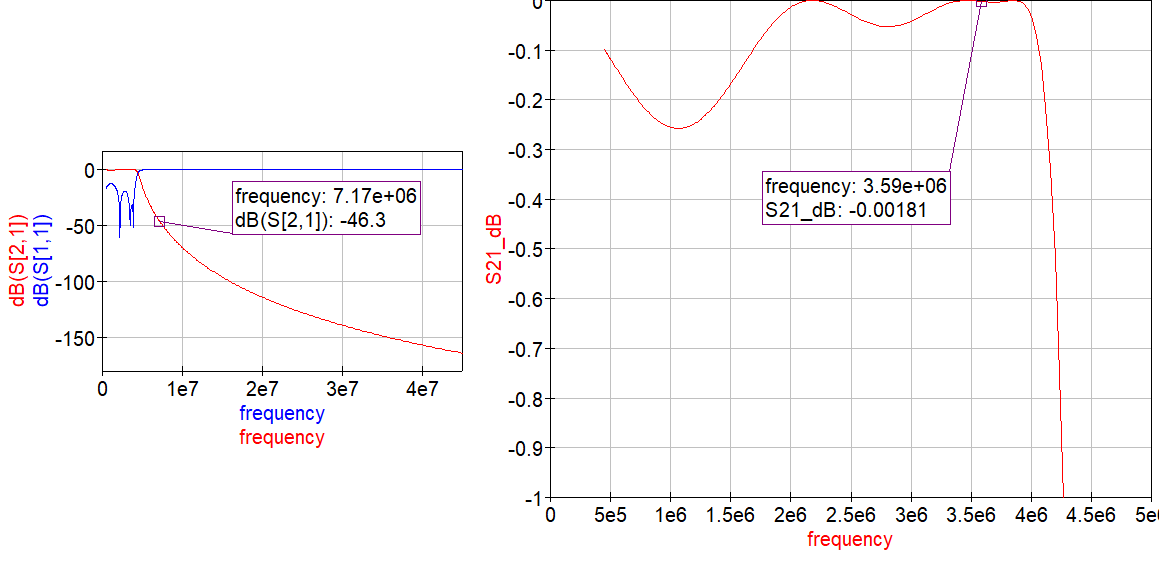
\includegraphics[scale=0.6]{res/TP_Simulation.png}
    \caption{Frequenzgang des Filters: Transmission in rot, Reflektionsfaktor in blau}
\end{figure}
Die Simulation zeigt das gewünschte Verhalten des Filters: Bei der gewünschten
Sendefrequenz von $3,5795$MHz beträgt die Dämpfung quasi $0$dB.
Die für uns eigentlich unkritische Welligkeit bleibt unter $-0.3$dB.

\subsection{Steuerung}
Der Sender wir von einem einfachen Mikrocontroller gesteuert. Dieser muss nur
sehr geringe Anforderungen erfüllen, da er keine aufwendigen Berechnungen oder anderweitige
Aufgaben bewältigen muss. Er muss lediglich in der Lage sein, Daten, wie z.B. das 
zu sendende Morsezeichen und die Sendeintervalllänge zu speichern und später dann
den Sender periodisch zu aktivieren. Deshalb haben wir für den Mikrocontroller vom
Typ ATtiny44 entschieden, der alle Voraussetzungen erfüllt. Der Mikrocontroller bekommt
ein externes Clock-Signal vom Quarz-Oszillator, der eine höhere Präzision, als die interne
Clock hat. Diese Präzision ist wichtig, da sich sonst auf dauer die Sendeintervalle von
verschiedenen Sendern überlappen können. Der Mikrocontroller schaltet im Sendebetrieb den Sender
über einen GPIO-Pin und ein UND-Gatter jeweils eine gewisse Zeit ein und aus, je nach eingestelltem
Morsezeichen. Ist das Sendeintervall vorbei, wird der Sender bis zum nächsten Intervall komplett
deaktiviert.

Der Mikrocontroller wird komplett in C programmiert.
@TODO mehr generischen Text schreiben...
Der Mikrocontroller ist folgendermaßen beschaltet:

\begin{figure}[H]
    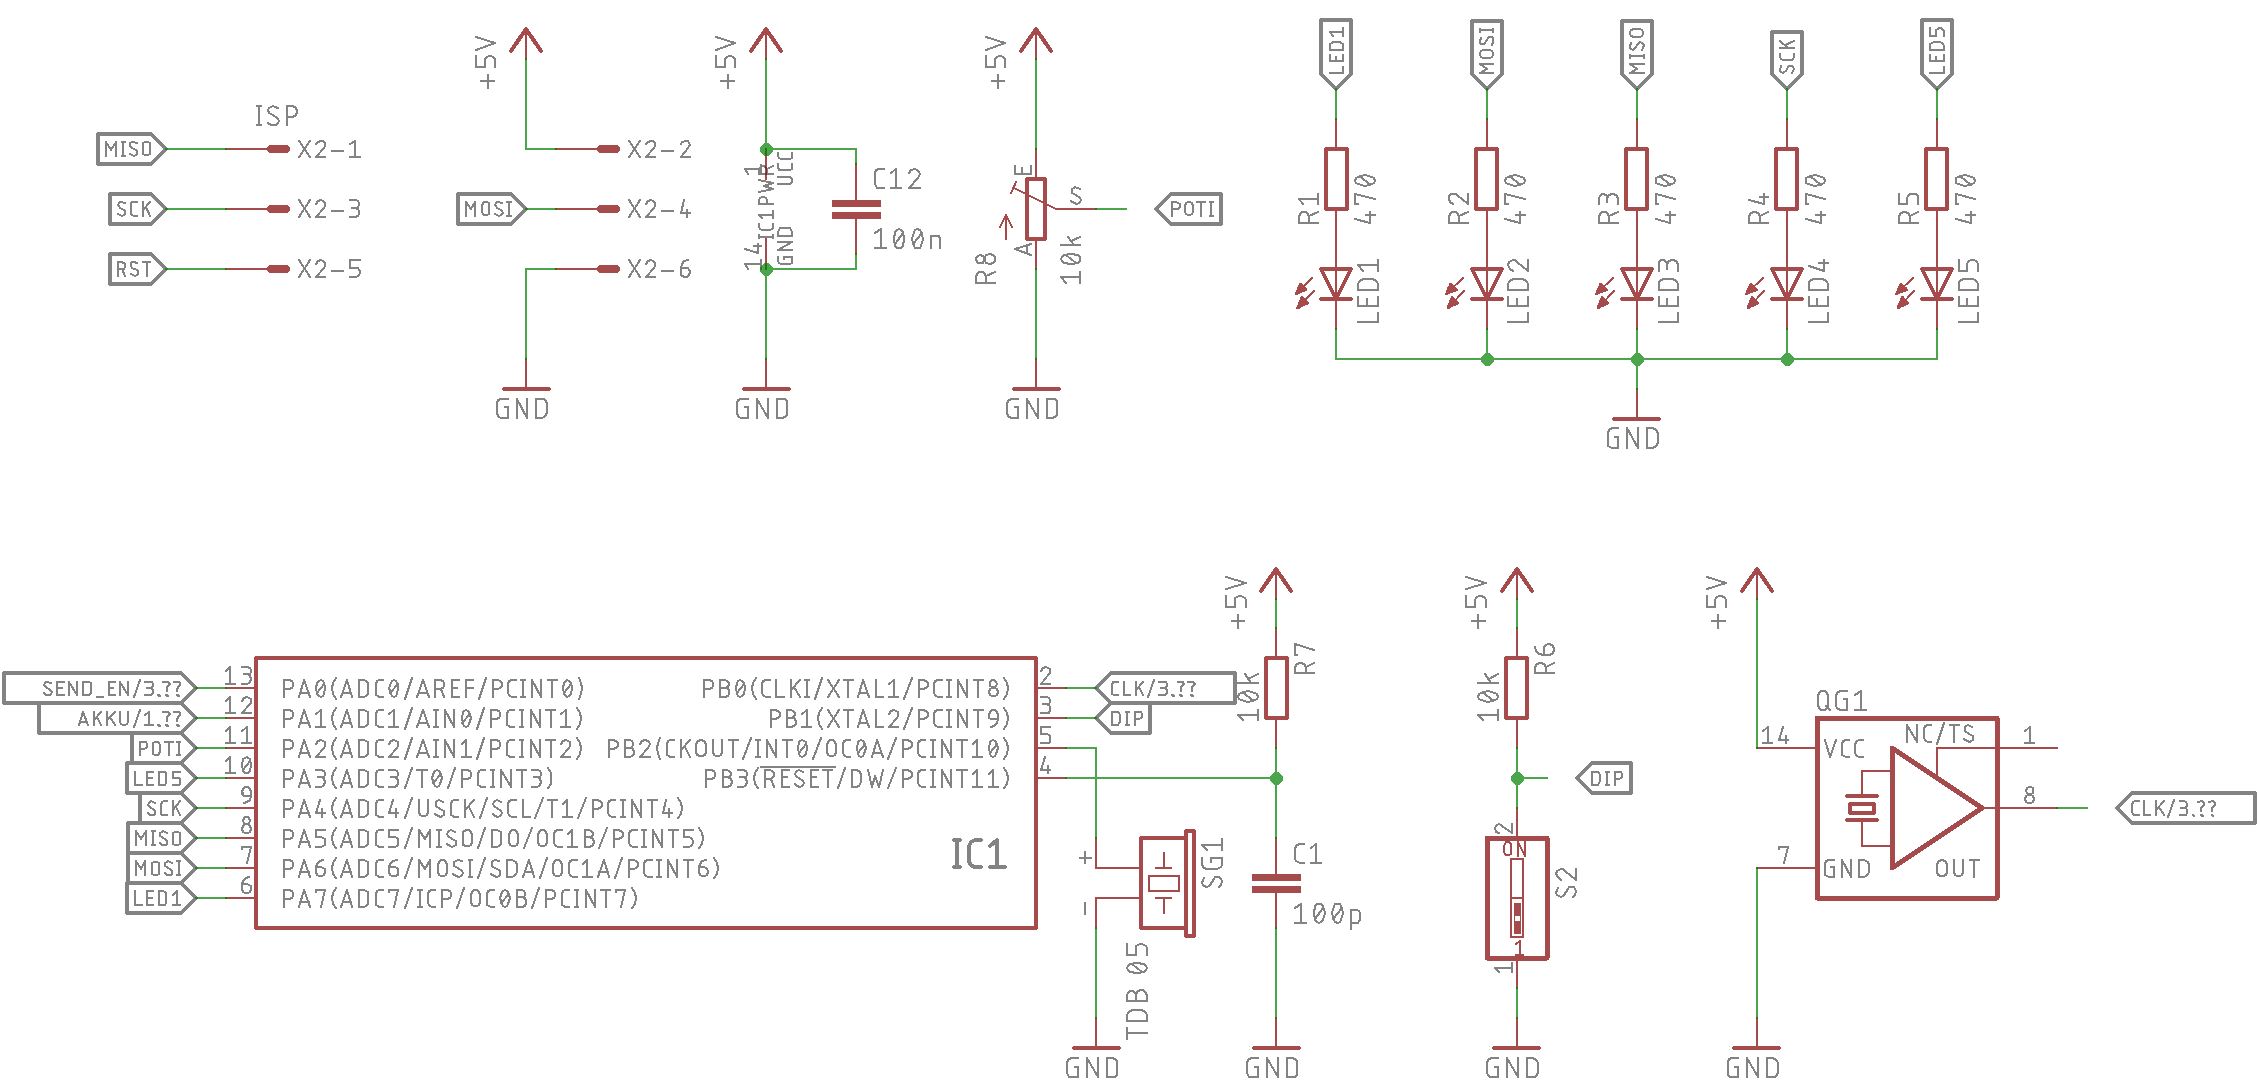
\includegraphics[scale=0.9]{res/Controller.png}
    \caption{Beschaltung des Mikrocontrollers}
\end{figure}

\subsection{Bedienung}
Der Fuchsjagd-Sender wird über einen Statusschalter, sowie über ein Potentiometer
gesteuert. Als Anzeige dienen 5 LEDs. Mit dem Statusschalter wird ausgewählt, ob
man das zu sendende Morsezeichen oder die Sendepausen einstellen möchte.
Mit dem Potentiometer wir der eigentliche Wert eingestellt. Über die LEDs wird dieser
Wert in bestimmten Schritten angezeigt. Einmal eingestellt, sendet der Sender das gewünschte
Morsezeichen in den festgelegten Zeitabständen für jeweils eine feste Zeitdauer. 
@TODO Konkretisieren! Wie groß sind die Wertschritte?!!!